%%%%%%%%%%%%%%%%%%%%%%%%%%%%%%%%%%%%%%%%%%%%%%%%%%%%%
% COPULAS
%%%%%%%%%%%%%%%%%%%%%%%%%%%%%%%%%%%%%%%%%%%%%%%%%%%%%
\subsection{Copula-Based Dependence Modeling}

%==============[	  Transition  ]==============
The sparse synthetic control framework provides an adaptive mechanism to construct a replicating portfolio that dynamically identifies influential assets from a broad candidate pool. However, the efficacy of a pairs trading strategy depends not only on accurate synthetic replication but also on quantifying how --and to what extent-- the target and synthetic assets co-move under varying market conditions. 
%
Traditional pairs-trading approaches often rely on linear correlation or cointegration measures, but these methods impose restrictive assumptions about the joint distribution of returns. Such assumptions are frequently violated in practice, particularly during periods of market stress where asymmetric tail dependencies and non-linear dynamics dominate.

To overcome these limitations, we complement the synthetic asset construction with copula-based dependence modeling. Copulas provide a flexible framework to decouple marginal distributions from the joint dependence structure, enabling us to capture non-linear and tail-dependent interactions that linear correlations overlook, model time-varying dependencies without assuming Gaussianity or stationarity and quantify conditional mispricing probabilities in a distributionally robust manner.
%
We now formalize the copula framework and its integration with the synthetic asset returns.

%==============[	  Introduction to bivariate copulas  ]==============
Let $(\Omega, \mathcal{F}, \mathbb{P})$ be a probability space and let $R, R^*: \Omega \to \mathbb{R}$ be real-valued random variables representing the target and synthetic log-returns, respectively, 
%where $R_t = y_t - y_{t-1}$ and $R^*_t = y^*_t - y^*_{t-1}$. 
Let $F_R$ and $F_{R^*}$ denote their respective cumulative distribution functions (CDFs).

%==============[	  Definition: Bivariate Copula  ]==============
\begin{definition}[Bivariate copula]
A bivariate copula is a function $C: [0,1]^2 \to [0,1]$ satisfying:
\begin{enumerate}
   \item $C(u,0) = C(0,v) = 0$ and $C(u,1) = u$, $C(1,v) = v$ for all $u,v \in [0,1]$ (boundary conditions)
   \item $C(u_2,v_2) - C(u_2,v_1) - C(u_1,v_2) + C(u_1,v_1) \geq 0$ for all $u_1 \leq u_2$, $v_1 \leq v_2$ in $[0,1]$ (2-increasing)
\end{enumerate}
\end{definition}

The fundamental relationship between copulas and joint distributions is established by Sklar's theorem:

%==============[	  Sklar's Theorem  ]==============
\begin{theorem}[Sklar (1959)]
Let $F_{R,R^*}$ be the joint CDF of $(R,R^*)$. Then there exists a bivariate copula $C: [0,1]^2 \to [0,1]$ such that
\begin{equation}
   F_{R,R^*}(r,r^*) = C(F_R(r), F_{R^*}(r^*)) \quad \forall r,r^* \in \mathbb{R}.
\end{equation}
If $F_R$ and $F_{R^*}$ are continuous, then $C$ is unique. Conversely, if $C$ is a copula and $F_R$, $F_{R^*}$ are CDFs, then $F_{R,R^*}$ defined above is a joint CDF with margins $F_R$ and $F_{R^*}$.
\end{theorem}
%
When uniqueness holds, the copula can be expressed through the probability integral transform: 
$$
C(u,v) = \mathbb P( F_R(R) \leq u, F_{R^*}(R^*) \leq v) 
\quad \text{for} \quad
(u,v)\in[0,1]^2
.
$$
The corresponding copula density $c:[0,1]^2\to\mathbb R_+$, when it exists, is given by
%When the joint CDF $F_{R,R^*}$ has a density $f_{R,R^*}$ and the copula $C$ is twice differentiable, the copula density is given by
$
   c(u,v) = \frac{\partial^2 C(u,v)}{\partial u \partial v},
%   c(u,v) = \partial^2 C(u,v) / \partial u \partial v
$
and the joint density can be expressed as
$
   f_{R,R^*}(r,r^*) = c(F_R(r), F_{R^*}(r^*)) f_R(r)f_{R^*}(r^*),
$
where $f_{R,R^*}$ is the joint density and $f_R$ and $f_{R^*}$ are the marginal densities.

Intuitively, Sklar's theorem tells us that any joint distribution can be decomposed into two parts: the marginal distributions of individual variables and a copula that captures their dependence structure. 
%This decomposition is particularly valuable for our pairs trading application as it allows us to separately model the behavior of individual assets and their joint dynamics.
This decomposition provides a framework for modeling the dependence structure between the target and synthetic returns independently of their marginal distributions. The implementation involves three stages: (1) nonparametric estimation of the marginal CDFs $F_R$, $F_{R^*}$ , (2) copula calibration from parametric classes $\mathcal{C} = \{C_\theta : \theta \in \Theta\}$ via maximum likelihood estimation, and (3) selection of an appropriate copula family 



%%%%%%%%%%%%%%%%%%%%%%%%%%%%%%%%%%%%%%%%%%%%%%%%%%%%%
\subsubsection{Marginal Distribution Estimation}
%%%%%%%%%%%%%%%%%%%%%%%%%%%%%%%%%%%%%%%%%%%%%%%%%%%%%

%\cite{Marti2016}

The foundation of copula modeling lies in the accurate estimation of marginal distributions for both target and synthetic asset returns. To maintain flexibility and avoid restrictive parametric assumptions, we adopt a non-parametric approach through empirical cumulative distribution functions (ECDFs).

%==============[	  Building Returns  ]==============
First, we construct logarithmic return series for both assets. Let $y_t$ and $y_t^*$ denote the log-prices of the target and synthetic assets at time $t$, respectively. The log-returns are computed as  
$
r_t = y_t - y_{t-1} 
%\quad 
~\text{and}~ 
%\quad 
r_t^* = y_t^* - y_{t-1}^* 
%\quad 
~\text{for}\ t = 2,\ldots,T,
$  
delivering return time series $\{r_t\}_{t=2}^T$ and $\{r_t^*\}_{t=2}^T$ for the target and stationary assets respectively. 

%==============[	  ECDFs  ]==============
Next, we estimate the empirical margins nonparametrically following Deheuvels (1979)'s normalized rank transform: 
%Next, we estimate the marginal distributions through linearly interpolated ECDFs. For any $r \in \mathbb{R}$, the empirical distribution functions are given by  
$$
\hat{F}_{R}(r) = \frac{1}{T-1} \sum_{t=2}^T \I{r_t \leq r} \quad \text{and} \quad \hat{F}_{R^*}(r^*) = \frac{1}{T-1} \sum_{t=2}^T \I{r_t^* \leq r^*},
$$  
where $\mathbb{I}(\cdot)$ denotes the usual indicator function. Following \cite{hudsonthames2024}, we then enforce linear interpolation between observed returns to ensure continuity of the distribution functions across their support. Also, to mitigate numerical instabilities during subsequent copula estimation, we constrain the ECDF outputs within $[\epsilon, 1-\epsilon]$ where $\epsilon = 10^{-5}$, thereby avoiding boundary effects at the distribution tails.

%==============[	  Probability Integral Transform  ]==============
The final step involves applying the probability integral transform to obtain uniform marginals. Specifically, we compute pseudo-observations  
$$
u_t = \hat{F}_R(r_t) \quad \text{and} \quad v_t = \hat{F}_{R^*}(r_t^*) \quad \text{for}\ t = 2,\ldots,T,
$$  
yielding paired realizations $(\mbf {u,v})=\{(u_t,v_t)\}_{t=2}^T$ that reside in the unit square $[0,1]^2$. This transformation, justified by Sklar's Theorem, effectively decouples the marginal distributions from the dependence structure. The resulting uniform variates serve as canonical inputs for copula specification while preserving the essential dependence characteristics between target and synthetic returns. 

%This non-parametric approach to marginal distribution estimation provides several advantages: it circumvents potential misspecification risks from parametric assumptions, maintains consistency with the empirical properties of financial returns, and ensures numerical stability during subsequent copula calibration stages. The procedure aligns with the canonical copula framework by construction, as the uniform pseudo-observations directly satisfy the requirements of Sklar's representation.


\cref{fig:all_CDFs_comparison} presents a comparative analysis of the empirical cumulative distribution functions (ECDFs) between the target and synthetic assets across both training and testing periods, revealing several notable patterns. The analysis of ECDFs in both return and price spaces provides crucial insights into the effectiveness of our synthetic replication strategy.
In the training period (top panels), we observe an almost perfect alignment between the target (red) and synthetic (blue) ECDFs in both return and price spaces. The log-returns distributions (top-left) exhibit the characteristic S-shaped curve typical of financial returns, with steep slopes around zero and thinner tails, suggesting that both assets capture similar distributional properties including volatility patterns and extreme events. The log-price ECDFs (top-right) show an equally strong correspondence, indicating successful replication of the price level dynamics during the training phase.
However, the testing period (bottom panels) reveals a striking contrast between returns and prices that has important implications for our trading strategy. The log-returns ECDFs (bottom-left) maintain their strong alignment, with both target and synthetic assets continuing to share nearly identical distributional properties. This persistence in the return space is particularly noteworthy as it suggests that our synthetic construction preserves its ability to mimic the target's return dynamics even out-of-sample.
In contrast, the log-price ECDFs (bottom-right) exhibit notable divergence in the testing period, especially in the upper quantiles (above the 0.6 probability level). This divergence manifests as a systematic deviation between the target and synthetic price paths, with the synthetic asset generally showing lower price levels than the target for given probability levels. This pattern suggests that while the return dynamics remain well-matched, price levels can drift apart over time due to the cumulative effect of small return differences.
This asymmetric behavior between returns and prices provides strong empirical justification for our copula-based approach, which focuses on modeling return dependencies rather than price-level relationships. The stability of the return distributions, even when price levels diverge, indicates that return-based trading signals may offer more reliable indicators of relative mispricings than traditional price-level methods. Furthermore, the observed price divergence in the testing period actually represents potential trading opportunities, as it suggests periods where the target and synthetic assets have moved out of their historical relationship, potentially creating conditions for profitable mean reversion trades.

%==============[	  Figure 2  ]==============
\inserthere{fig:all_CDFs_comparison}
\begin{figure}[H]
  \caption{Empirical Cumulative Distribution Functions of Target and Synthetic Assets}
  \centering
  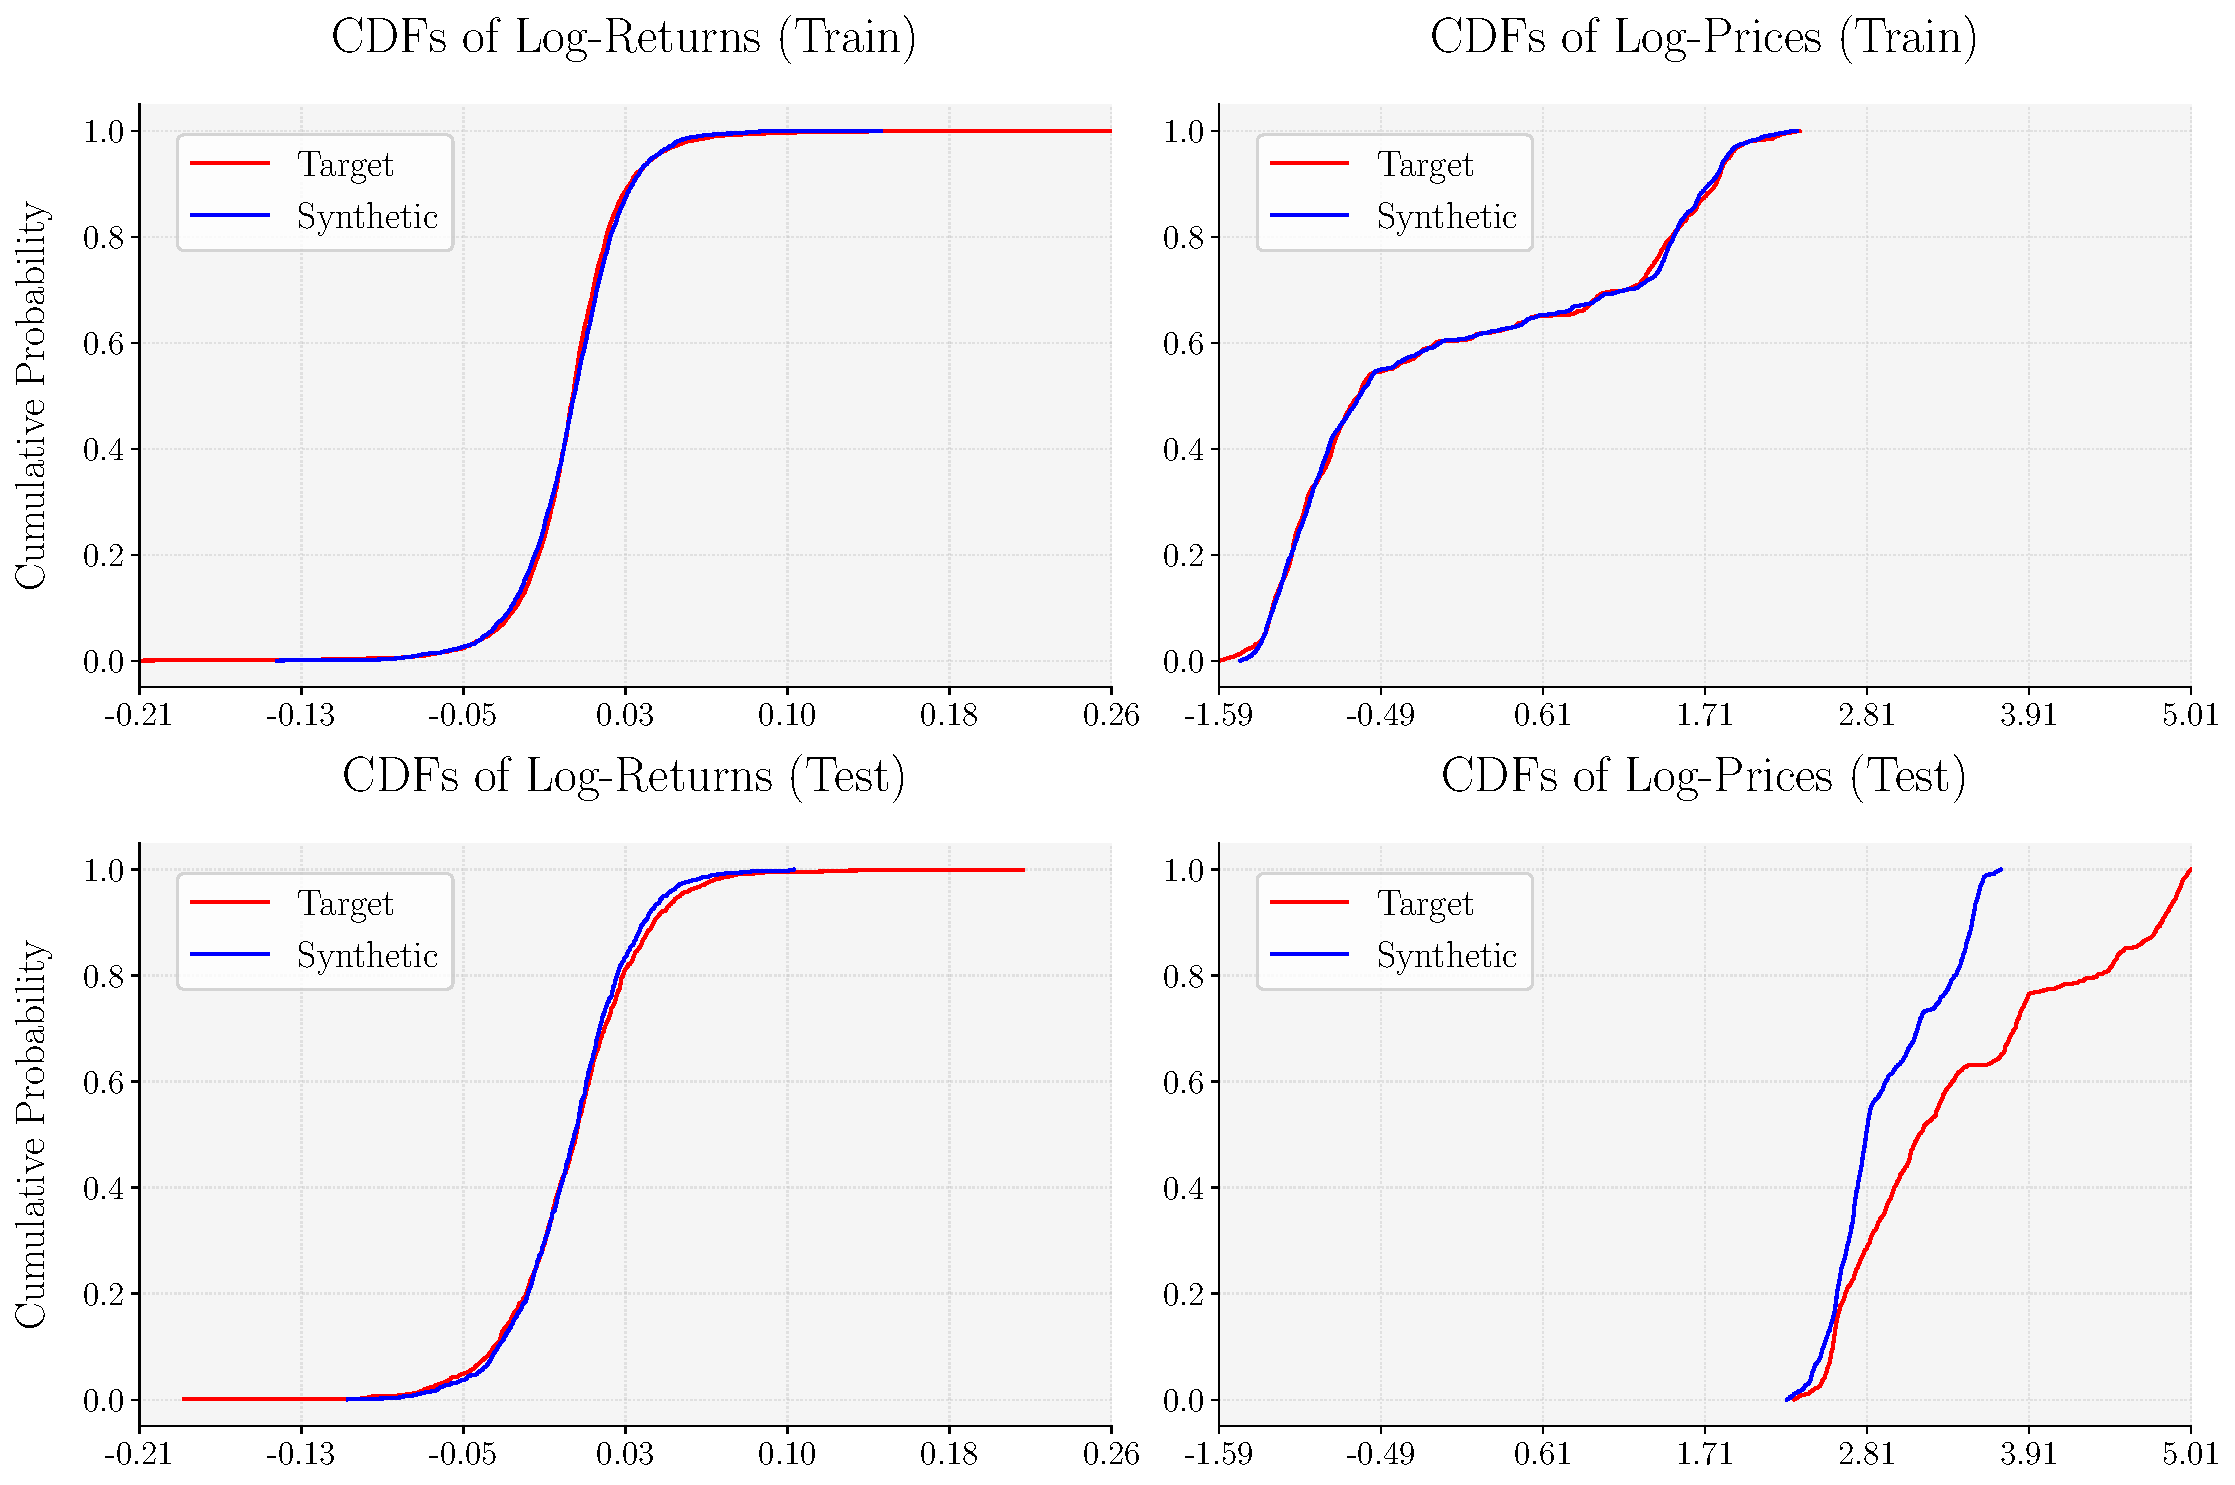
\includegraphics[scale=0.47]{/Users/jesusvillotamiranda/Library/CloudStorage/OneDrive-UniversidaddeLaRioja/GitHub/Repository/arbitragelab-master/__OUTPUT_TeX__/figures/all_CDFs_comparison.pdf}
  \label{fig:all_CDFs_comparison}
%.............
\vspace{0.5cm}
\begin{minipage}{\textwidth}
\setlength{\parindent}{0pt}
\small\textit{Note: 
This figure presents the linearly interpolated empirical cumulative distribution functions (ECDFs) for both log-returns and log-prices of the target (red) and synthetic (blue) assets. The panels are divided into training period (top) and test period (bottom). The left panels show the CDFs of daily log-returns, while the right panels display the CDFs of log-price levels. The y-axis represents cumulative probability from 0 to 1, and the x-axis shows the corresponding log-returns or log-prices."
}
\end{minipage}
%.............
\end{figure}

\bblue{
We then estimate the empirical copula: 
$$
C_n(u,v) = \frac{1}{T-1} \sum_{t=2}^T \I{u_t\leq u, v_t \leq v},
$$
for the pseudo-observations of returns and prices.}
%
\cref{fig:CDF_scatter_comparison} reveals several important patterns in the relationship between target and synthetic assets across different dimensions. In the returns series (left panels), we observe considerable dispersion around the 45-degree line in both training and testing periods, with points forming a cloud-like pattern that suggests a consistent dependency structure. This dispersion reflects the inherent volatility in daily returns, yet the overall symmetric pattern around the diagonal indicates that the synthetic asset effectively captures the statistical properties of the target's return distribution.

The price series (right panels) exhibits markedly different behavior. During the training period, we observe a tight clustering of points along the diagonal, indicating that the synthetic asset closely tracks the price level distribution of the target. However, the testing period reveals a subtle but important deviation from this pattern, with increased dispersion and slight systematic deviations from the 45-degree line, particularly in the middle range of the distribution (0.4-0.6 probability region). This divergence suggests that while the synthetic asset maintains similar distributional properties in returns space, the accumulated price levels begin to show some drift in the out-of-sample period.

The contrast between return and price space behaviors is particularly instructive. The relatively stable pattern in returns space, even during the testing period, suggests that the copula-based approach successfully captures the underlying return dynamics. Meanwhile, the gradual price divergence in the testing period highlights the challenges of maintaining long-term price level correspondence between target and synthetic assets, a common phenomenon in pairs trading that often creates trading opportunities.

This dual perspective-stability in returns but drift in prices-provides empirical support for our strategy's focus on return-based copula modeling rather than price-level relationships, as it appears to offer more robust statistical properties for trading signal generation.

%==============[	  Figure 3  ]==============
\inserthere{fig:CDF_scatter_comparison}
\begin{figure}[H]
  \caption{Empirical copula distribution for Returns and Prices}
%  \caption{Scatter Plots of CDF Pairs for Target and Synthetic Assets}
  \centering
  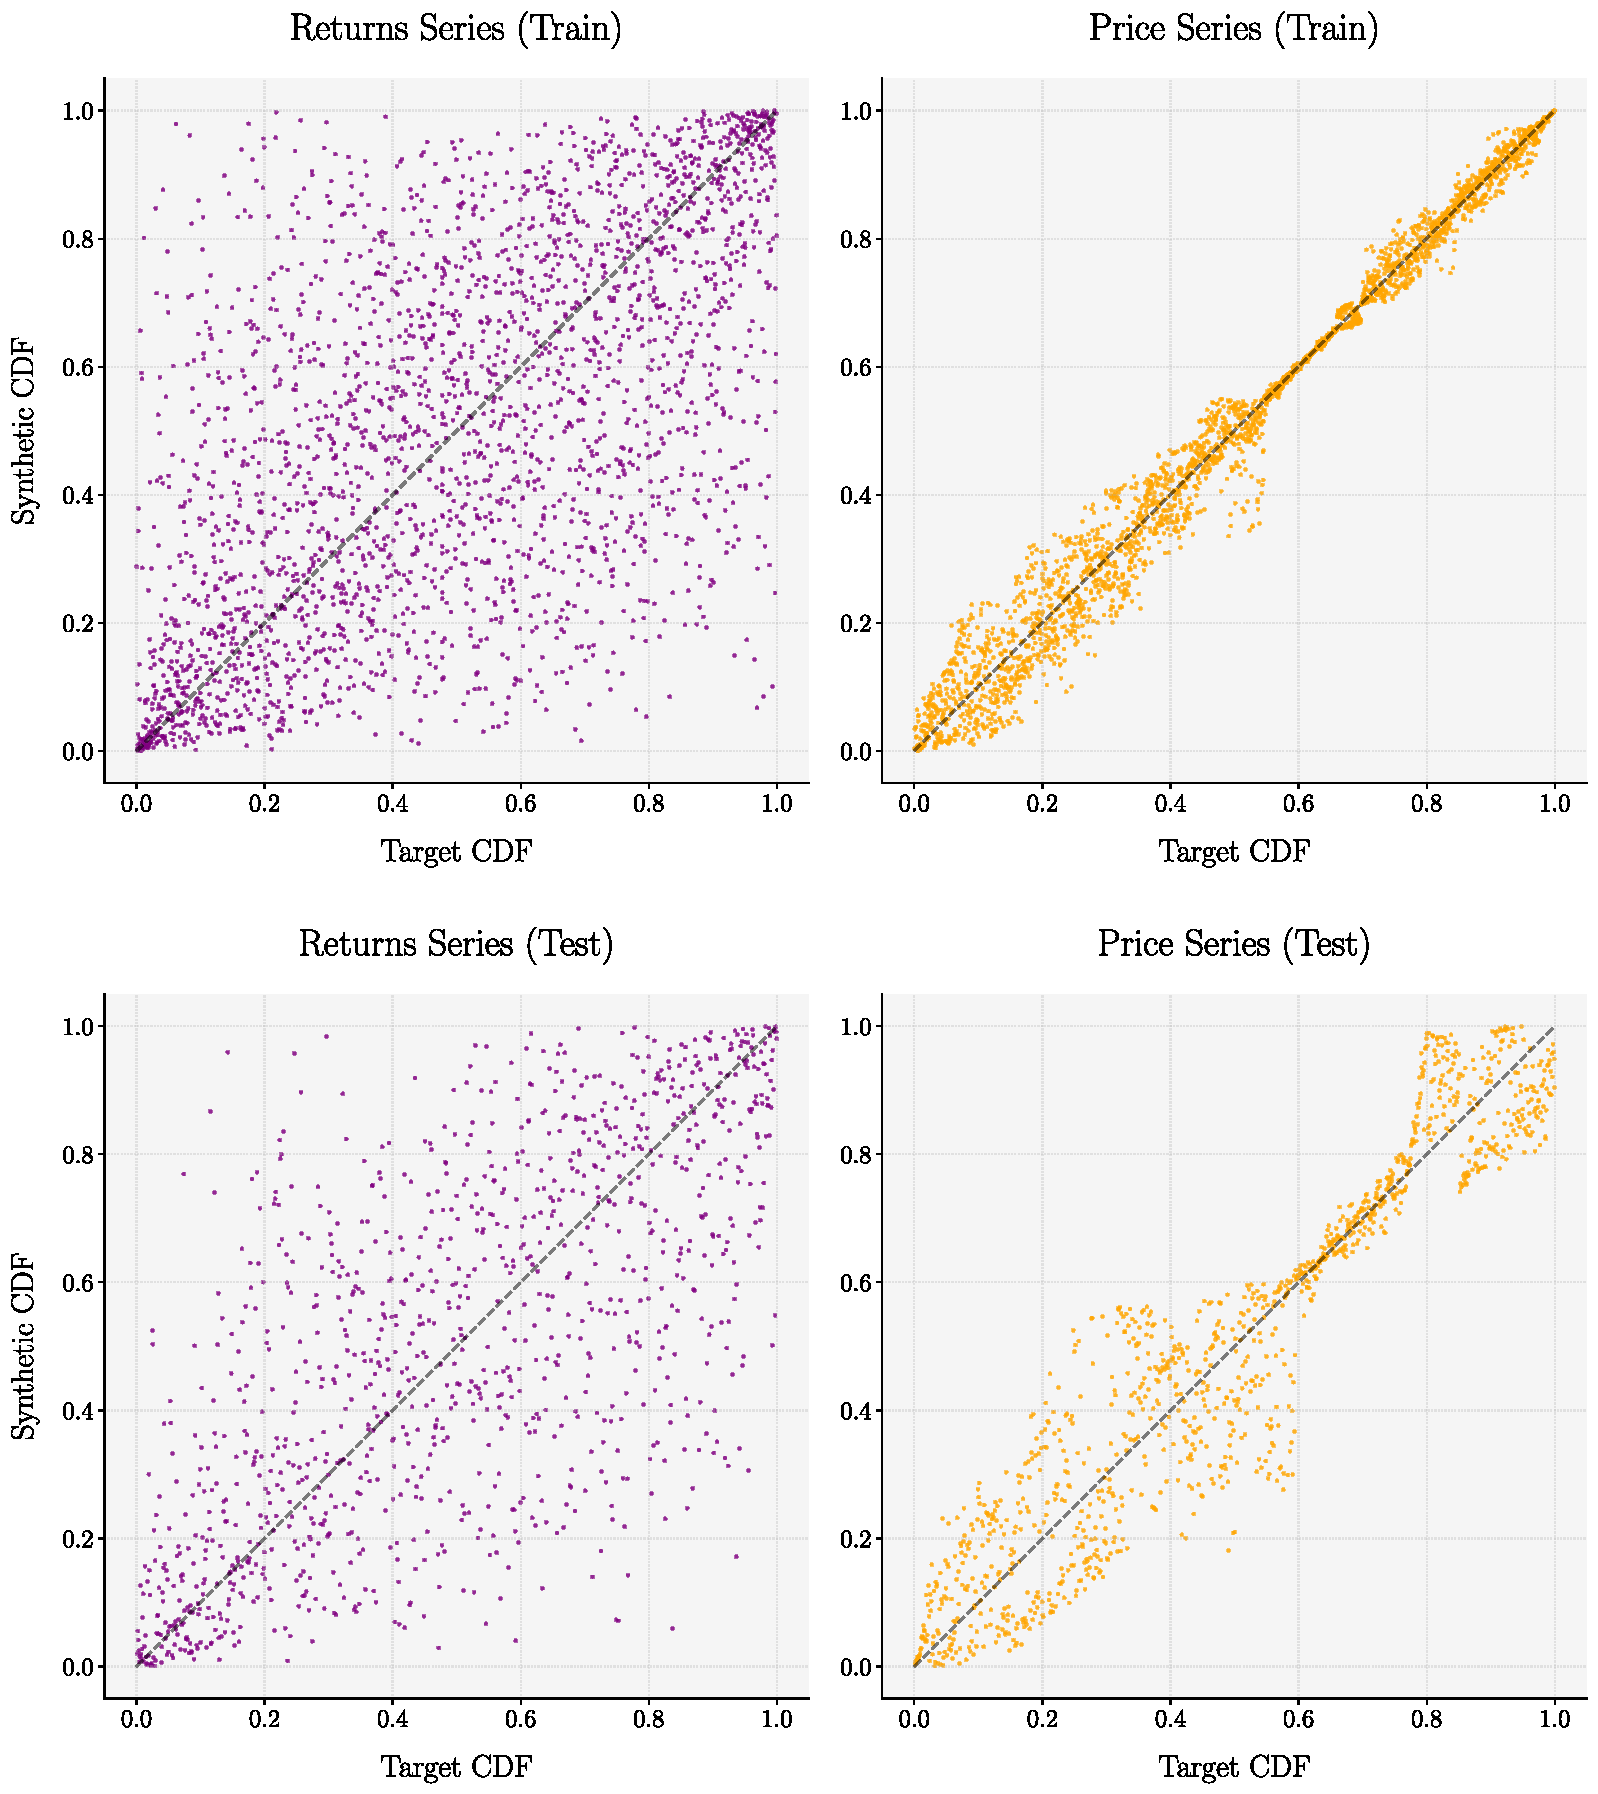
\includegraphics[scale=0.4]{/Users/jesusvillotamiranda/Library/CloudStorage/OneDrive-UniversidaddeLaRioja/GitHub/Repository/arbitragelab-master/__OUTPUT_TeX__/figures/CDF_scatter_comparison.pdf}
  \label{fig:CDF_scatter_comparison}
%.............
\vspace{0.5cm}
\begin{minipage}{\textwidth}
\setlength{\parindent}{0pt}
\footnotesize\textit{Note: 
Scatter plots comparing the cumulative distribution functions (CDFs) of the target asset and the synthetic asset for both returns and prices during training and testing periods. The top row displays the CDFs for the training data, while the bottom row shows the CDFs for the testing data. The left column represents the returns series, and the right column represents the price series. Each plot compares the target CDF (x-axis) against the synthetic CDF (y-axis). Both axes represent the [0,1] probability space of the copula domain, with values extending slightly beyond this range to show boundary behavior. The close alignment of points along the diagonal line indicates a strong similarity between the target and synthetic distributions. The returns series exhibit more dispersion, reflecting the volatility in returns, while the price series show a tighter fit, suggesting that the synthetic asset effectively replicates the price dynamics of the target asset.
}
\end{minipage}
%.............

\end{figure}


%%%%%%%%%%%%%%%%%%%%%%%%%%%%%%%%%%%%%%%%%%%%%%%%%%%%%
\subsubsection{Copula calibration from parametric classes}
%%%%%%%%%%%%%%%%%%%%%%%%%%%%%%%%%%%%%%%%%%%%%%%%%%%%%

We consider parametric copula families $\mathcal{C} = \{C_\theta : \theta \in \Theta\}$. Each copula $C_{\theta}$ is calibrated to the training data using the algorithms detailed in \cref{subsec:copula_calibration}.  In the class of elliptical copulas, we consider the Gaussian and Student-$t$ copulas. The Gaussian copula is calibrated by obtaining the empirical covariance matrix of the gaussianized pseudo-observations, while the Student-$t$ copula is calibrated by choosing the degrees of freedom that maximize the likelihood (and consequently obtaining the correlation parameter associated to the empirical covariance matrix fitted from the studentized pseudo-observations). In the Archimedean class, we consider the Clayton, Gumbel, Frank, Joe and N14 copula. The calibration of these copulas relies on inverting the relationship between Kendall's tau and their generators.

%==============[	  OLD WRITEUP: MAXIMUM LIKELIHOOD (wrong!) ]==============
%The goal of copula fitting is to find the copula that best describes the dependence structure between the returns of the target and synthetic assets. This is done by maximizing the likelihood of the observed data under different copula models. 
%%Let $(\mbf u, \mbf v)=[(u_t, v_t)]_{t=1}^T$ be the pseudo-observations obtained through the marginal transformation process, where $u_t = \hat{F}_R(r_t)$ and $v_t = \hat{F}_{R^*}(r_t^*)$. 
%We consider parametric copula families $\mathcal{C} = \{C_\theta : \theta \in \Theta\}$ where each copula $C_\theta$ has density
%$
%%\begin{equation} \label{eq:copula_density_def}
%c_\theta(u,v) = \frac{\partial^2 C_\theta}{\partial u \partial v}(u,v)
%%\end{equation}
%.
%$
%%\subsubsection{Maximum Likelihood Estimation}
%For each candidate copula family, we estimate parameters via constrained maximum likelihood:
%%
%\begin{equation} \label{eq:mle}
%\hat{\theta} = \argmax_{\theta \in \Theta} \ell(\theta | \mbf {u,v}) \quad \text{where} \quad 
%\ell(\theta| \mbf {u,v}) := \sum_{t\in\mathcal T_{tr}} \log c_\theta(u_t, v_t)
%.
%\end{equation}
%%
%The optimization is subject to parameter constraints $\Theta$ specific to each copula family (a formal description of the copula fitting procedure can be found in \cref{alg:copula_fit}):
%----------------------------------------------------

\cref{fig:copula_samples_comparison} visualizes the dependence structures of different parametric copula families through density heatmaps generated from samples. The sampling procedures are detailed in \cref{subsec:copula_sampling}. The Archimedean copulas each exhibit distinct characteristics: Clayton demonstrates strong lower tail dependence, Gumbel and Joe show pronounced upper tail dependence, while Frank captures dependence concentrated in both tails. Among elliptical copulas, the Gaussian shows symmetric dependence with moderate tails, while the Student-t accommodates heavier tails in both directions. The N14, as a Clayton-Gumbel mixture, combines properties of both families to achieve a more flexible dependence structure. These varying patterns underscore how each family could potentially capture different aspects of movement between the target and synthetic asset.

%==============[	  Figure 4  ]==============
\inserthere{fig:copula_samples_comparison}
\begin{figure}[H]
  \caption{Copula Density Heatmaps for Different Parametric Families}
  \centering
  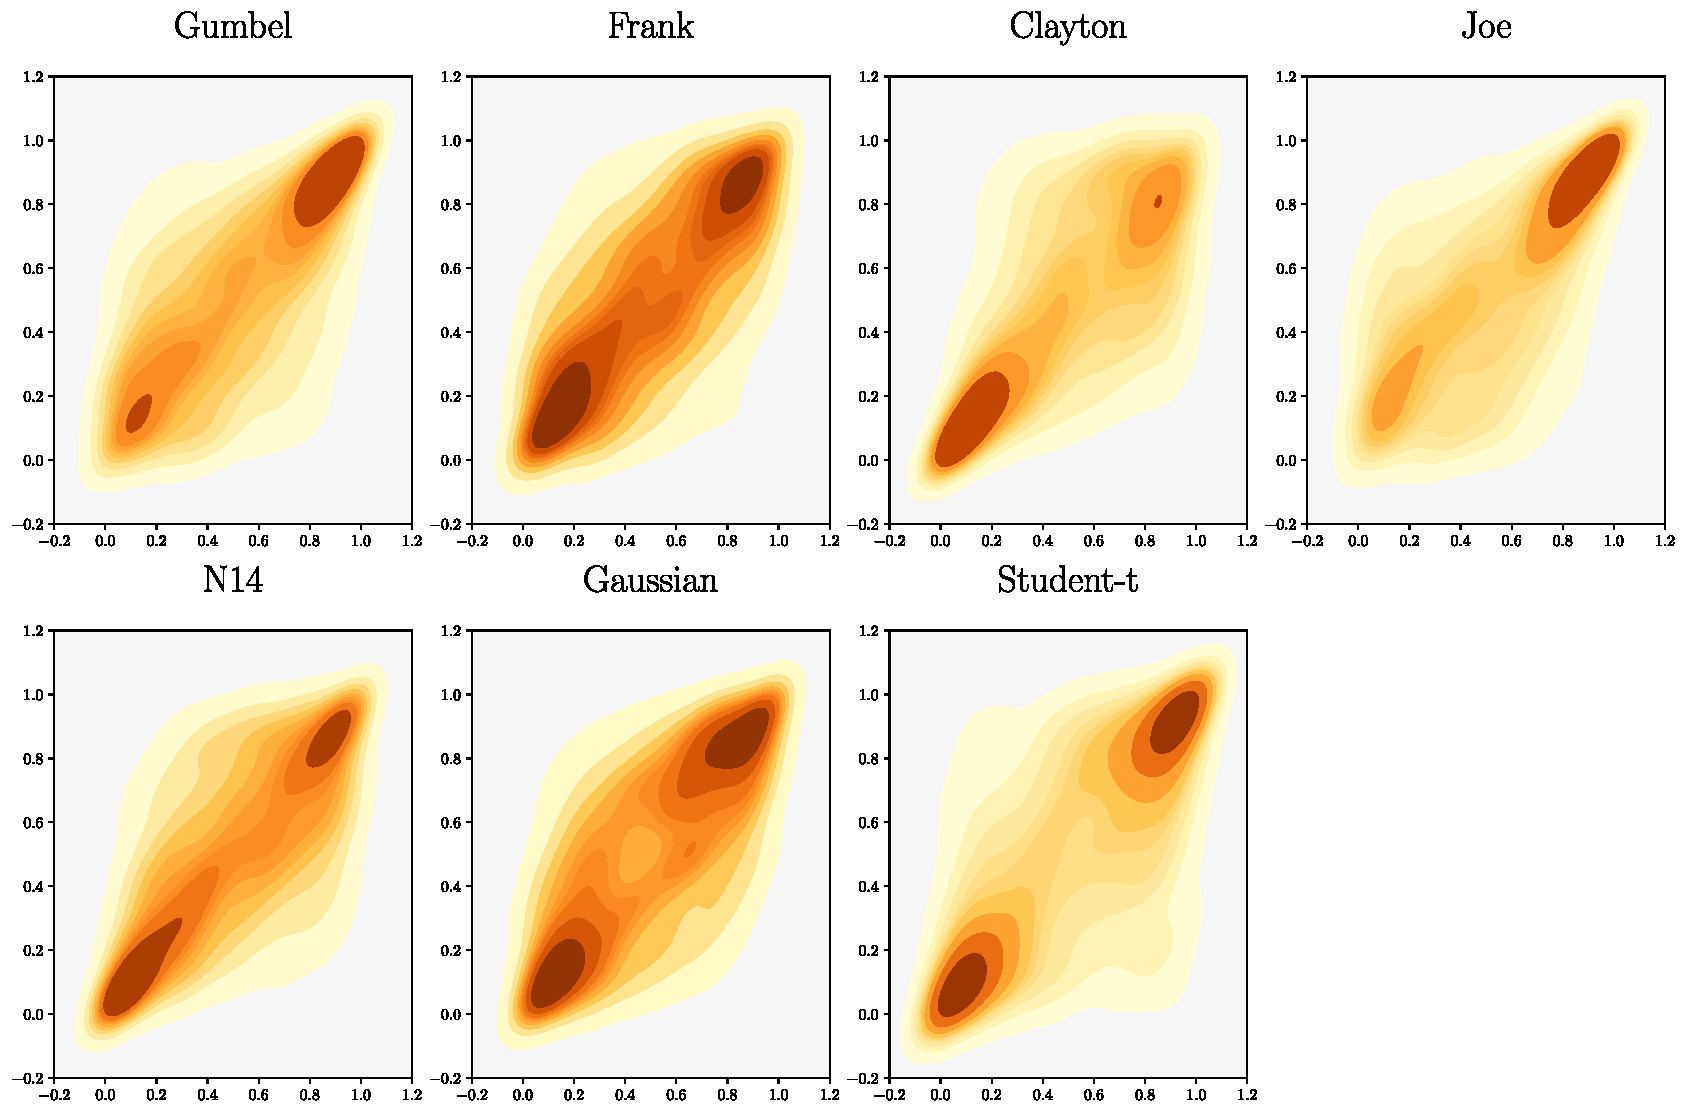
\includegraphics[scale=0.47]{/Users/jesusvillotamiranda/Library/CloudStorage/OneDrive-UniversidaddeLaRioja/GitHub/Repository/arbitragelab-master/__OUTPUT_TeX__/figures/copula_samples_comparison.pdf}
  \label{fig:copula_samples_comparison}
%.............
\vspace{0.5cm}
\begin{minipage}{\textwidth}
\setlength{\parindent}{0pt}
\small\textit{Note: 
Contour plots of copula densities for various parametric families, illustrating the dependence structures between the target and synthetic asset returns. Each subplot represents a different copula family: Gumbel, Frank, Clayton, Joe, N14, Gaussian, and Student-t. The color intensity in the plots indicates the density of the copula, with darker regions representing higher densities. These visualizations highlight the differences in tail dependencies and overall dependence structures captured by each copula family. The Gumbel and Clayton copulas exhibit stronger upper and lower tail dependencies, respectively, while the Gaussian copula shows symmetric dependencies. The Student-t copula accounts for heavier tails, and the Frank copula displays a balanced dependence structure. 
}
\end{minipage}
%.............

\end{figure}

%%%%%%%%%%%%%%%%%%%%%%%%%%%%%%%%%%%%%%%%%%%%%%%%%%%%%
\subsubsection{Selection of an appropriate copula family}
%%%%%%%%%%%%%%%%%%%%%%%%%%%%%%%%%%%%%%%%%%%%%%%%%%%%%

After estimating parameters for each candidate copula family $\mathcal{C} = \{C_\theta : \theta \in \Theta\}$, we select the optimal model using information criteria that balance goodness-of-fit against model complexity. Let $\ell(\hat{\theta}|\mbf {u,v}) = \max_{\theta\in\Theta} \sum_{t\in\mathcal T_{tr}} \ln c_{{\theta}}(u_t, v_t)$ be the in-sample maximized log-likelihood for a copula with parameter estimate $\hat{\theta}$, where $T_{tr}:=\card{\mathcal T_{tr}}$ is the sample size and $k$ is the number of parameters. 
The densities for each copula family are given in \cref{subsec:copula_densities}.
We evaluate the following information criterions:
$$
\begin{array}{lllll}
\text{\textit{Akaike}} &&& \text{AIC} &= [\fracc{2T_{tr}}{T_{tr}-k-1}] \cdot k - 2\ell(\hat{\theta}|\mathbf{u,v})
\\[0.44em]
\text{\textit{Schwarz/Bayesian}} &&& \text{SIC} &= k\ln(T_{tr}) - 2\ell(\hat{\theta}|\mathbf{u,v})
\\[0.44em]
\text{\textit{Hannan-Quinn}} &&& \text{HQIC} &= 2k\ln(\ln(T_{tr})) - 2\ell(\hat{\theta}|\mathbf{u,v})
\end{array}
$$
%$$
%\begin{array}{lllll}
%\text{\textit{Akaike}} &&& \text{AIC} &= 2k - 2
%%\ell(\hat{\theta}) 
%\ell(\hat{\theta}|\mbf {u,v})
%\\
%\text{\textit{Schwarz/Bayesian}} &&& \text{SIC} &= k\ln(T-1) - 2
%%\ell(\hat{\theta}) 
%\ell(\hat{\theta}|\mbf {u,v})
%\\
%\text{\textit{Hannan-Quinn}} &&& \text{HQIC} &= 2k\ln(\ln T-1) - 2
%%\ell(\hat{\theta})
%\ell(\hat{\theta}|\mbf {u,v})
%\end{array}
%$$

The copula family with the lowest value for a chosen criterion is selected as optimal. These criteria penalize overfitting through the $k$ term while rewarding better fit through the log-likelihood.
%$\ell(\hat{\theta}|\mbf {u,v})$. 
% The SIC provides the strongest penalty for model complexity, making it particularly suitable for financial applications where parsimony is valued.

%The scatter plots of the empirical and fitted copulas reveal significant lower tail dependence in the returns, consistent with the increased correlation during market downturns. 


%==============[	  Table 2 ]==============
\inserthere{tab:copula_fit}
\begin{table}[H]
\centering
\caption{Copula Fitting Results}
\label{tab:copula_fit}
\begin{tabular}{lrrrr}
\toprule
Copula & SIC & AIC & HQIC \\
\toprule
Joe & -671.50 & -677.39 & -675.26 \\
Clayton & -1168.92 & -1174.80 & -1172.67 \\
Gumbel & -1210.02 & -1215.90 & -1213.78 \\
Frank & -1212.68 & -1218.56 & -1216.43 \\
Gaussian & -1337.69 & -1343.57 & -1341.44 \\
N14 & -1425.18 & -1431.06 & -1428.94 \\
Student & -1427.05 & -1432.94 & -1430.81 \\
\bottomrule
\end{tabular}
\label{tab:copula_fits}
%----------------------------------------------------
\vspace{0.5cm}
\begin{minipage}{\textwidth}
\setlength{\parindent}{0pt}
\small\textit{Note: 
This table reports goodness-of-fit measures for various copula specifications used to model the dependence structure between the target and synthetic asset returns. The evaluation metrics include the Schwarz Information Criterion (SIC), Akaike Information Criterion (AIC), and Hannan-Quinn Information Criterion (HQIC). All criteria balance model fit against complexity, with lower values indicating better models. The Student-t copula achieves the best fit across all three criteria, followed closely by the N14 mixed copula, suggesting that the dependence structure exhibits tail dependence and asymmetry.
}
\end{minipage}
%----------------------------------------------------
\end{table}

\cref{tab:copula_fit} presents the fitting results for different copula families.  The comparative analysis of copula specifications reveals a clear dominance of elliptical copulas in modeling the dependence structure between  our target and synthetic returns. The Student-t copula achieves the best fit across all information criteria, %(SIC: -1427.05, AIC: -1432.94, HQIC: -1430.81)
followed closely by the N14 mixed copula and the Gaussian copula, with substantially better performance than all Archimedean specifications. This hierarchy in goodness-of-fit measures, particularly the superior performance of symmetric specifications (Student-t, Gaussian) over asymmetric ones (Clayton, Gumbel, Joe), indicates that the dependence structure is predominantly symmetric, which aligns with the theoretical construction of the synthetic control as a tracking portfolio.

The significant improvement in fit from Gaussian to Student-t copula ($\Delta \t{SIC} \approx 90$ points) demonstrates that while symmetry is essential, the joint distribution exhibits heavier tails than implied by normal dependence. This finding is further supported by the Frank copula's performance, which achieves better fit than other Archimedean copulas but worse than elliptical specifications, suggesting that symmetric dependence without tail dependence is insufficient for capturing the full relationship. The relatively poor fit of copulas with exclusive lower tail (Clayton, SIC: -1168.92) or upper tail (Joe, SIC: -671.50) dependence reinforces that the target-synthetic relationship maintains its symmetric structure even during extreme market movements, a desirable property for the stability of our trading strategy.


